%%
%% This is file `sample-sigplan.tex',
%% generated with the docstrip utility.
%%
%% The original source files were:
%%
%% samples.dtx  (with options: `all,proceedings,bibtex,sigplan')
%% 
%% IMPORTANT NOTICE:
%% 
%% For the copyright see the source file.
%% 
%% Any modified versions of this file must be renamed
%% with new filenames distinct from sample-sigplan.tex.
%% 
%% For distribution of the original source see the terms
%% for copying and modification in the file samples.dtx.
%% 
%% This generated file may be distributed as long as the
%% original source files, as listed above, are part of the
%% same distribution. (The sources need not necessarily be
%% in the same archive or directory.)
%%
%%
%% Commands for TeXCount
%TC:macro \cite [option:text,text]
%TC:macro \citep [option:text,text]
%TC:macro \citet [option:text,text]
%TC:envir table 0 1
%TC:envir table* 0 1
%TC:envir tabular [ignore] word
%TC:envir displaymath 0 word
%TC:envir math 0 word
%TC:envir comment 0 0
%%
%% The first command in your LaTeX source must be the \documentclass
%% command.
%%
%% For submission and review of your manuscript please change the
%% command to \documentclass[manuscript, screen, review]{acmart}.
%%
%% When submitting camera ready or to TAPS, please change the command
%% to \documentclass[sigconf]{acmart} or whichever template is required
%% for your publication.
%%
%%
% \documentclass[sigconf,screen,review,anonymous]{acmart}
\documentclass[sigconf,screen]{acmart}
%%
%% \BibTeX command to typeset BibTeX logo in the docs
\AtBeginDocument{%
  \providecommand\BibTeX{{%
    Bib\TeX}}}

%% Rights management information.  This information is sent to you
%% when you complete the rights form.  These commands have SAMPLE
%% values in them; it is your responsibility as an author to replace
%% the commands and values with those provided to you when you
%% complete the rights form.
\setcopyright{none}
\copyrightyear{2026}
\acmYear{2026}
\acmDOI{}
%% These commands are for a PROCEEDINGS abstract or paper.
\acmConference[Under Review]{Manuscript Under Review}{2026}{TBD}
%%
%%  Uncomment \acmBooktitle if the title of the proceedings is different
%%  from ``Proceedings of ...''!
%%
%%\acmBooktitle{Woodstock '18: ACM Symposium on Neural Gaze Detection,
%%  June 03--05, 2018, Woodstock, NY}
\acmISBN{}


%%
%% Submission ID.
%% Use this when submitting an article to a sponsored event. You'll
%% receive a unique submission ID from the organizers
%% of the event, and this ID should be used as the parameter to this command.
%%\acmSubmissionID{123-A56-BU3}

%%
%% For managing citations, it is recommended to use bibliography
%% files in BibTeX format.
%%
%% You can then either use BibTeX with the ACM-Reference-Format style,
%% or BibLaTeX with the acmnumeric or acmauthoryear sytles, that include
%% support for advanced citation of software artefact from the
%% biblatex-software package, also separately available on CTAN.
%%
%% Look at the sample-*-biblatex.tex files for templates showcasing
%% the biblatex styles.
%%

%%
%% The majority of ACM publications use numbered citations and
%% references.  The command \citestyle{authoryear} switches to the
%% "author year" style.
%%
%% If you are preparing content for an event
%% sponsored by ACM SIGGRAPH, you must use the "author year" style of
%% citations and references.
%% Uncommenting
%% the next command will enable that style.
%%\citestyle{acmauthoryear}

\usepackage{multirow}
\usepackage{array}
\usepackage{stfloats}

%%
%% end of the preamble, start of the body of the document source.
\begin{document}

%%
%% The "title" command has an optional parameter,
%% allowing the author to define a "short title" to be used in page headers.
\title{CanonFuse3D: Human-Centric Canonical Fusion for Calibration-Free Dual-View 3D Pose Estimation in Skiing Videos}

%%
%% The "author" command and its associated commands are used to define
%% the authors and their affiliations.
%% Of note is the shared affiliation of the first two authors, and the
%% "authornote" and "authornotemark" commands
%% used to denote shared contribution to the research.
% \authornotemark[1]
% \authornote{Both authors contributed equally to this research.}

\author{Kaixu Chen}
\orcid{0009-0003-8698-8899}
\email{chenkaixusan@gmail.com}
\affiliation{%
  \institution{Center for Computational Sciences, University of Tsukuba}
  \city{Tsukuba}
  \state{Ibaraki}
  \country{Japan}
}

\author{Nan Luo}
\email{nan.luo@image.iit.tsukuba.ac.jp}
\orcid{0009-0000-6282-4070}
\affiliation{%
  \institution{Intelligent and Mechanical Interaction Systems, University of Tsukuba}
  \city{Tsukuba}
  \state{Ibaraki}
  \country{Japan}
}

\author{Chun Xie}
\email{xie.chun@image.iit.tsukuba.ac.jp}
\orcid{0000-0003-4936-7404}
\affiliation{%
  \institution{Center for Computational Sciences, University of Tsukuba}
  \city{Tsukuba}
  \state{Ibaraki}
  \country{Japan}
}

\author{Eiichi Naito}
\email{eiichi.naito@nict.go.jp}
\orcid{0000-0002-9509-813X}
\affiliation{%
 \institution{National Institute of Information and Communications Technology, Advanced ICT Research Institute}
 \city{Osaka}
%  \state{Arunachal Pradesh}
 \country{Japan}}

\author{Toshitaka Kimura}
\email{toshitaka.kimura@ntt.com}
\orcid{0000-0002-1334-3438}
\affiliation{%
  \institution{NTT Communication Science Laboratories}
  \city{Tokyo}
  % \state{}
  \country{Japan}}


\author{Itaru Kitahara}
\email{kitahara.itaru@image.iit.tsukuba.ac.jp}
\orcid{0000-0002-5186-789X}
\affiliation{%
  \institution{Center for Computational Sciences, University of Tsukuba}
  \city{Tsukuba}
  \state{Ibaraki}
  \country{Japan}
}
% \email{TODO: add author email}

%%
%% By default, the full list of authors will be used in the page
%% headers. Often, this list is too long, and will overlap
%% other information printed in the page headers. This command allows
%% the author to define a more concise list
%% of authors' names for this purpose.
\renewcommand{\shortauthors}{Chen et al.}

%%
%% The abstract is a short summary of the work to be presented in the
%% article.
\begin{abstract}
This paper presents a calibration-free dual-view 3D pose refinement framework for sports motion analysis. Monocular 3D pose estimators are practical for field videos, but they often suffer from depth ambiguity, viewpoint-dependent errors, self-occlusion, and temporal jitter, especially in fast sports such as skiing. Calibrated multi-view reconstruction can reduce these ambiguities, but accurate camera calibration is difficult to obtain in temporary or unconstrained sports recording environments. We therefore propose a post-estimation refinement framework in which two independently estimated 3D pose streams from left and right views are fused without using camera intrinsics or extrinsics.
% We therefore study a post-estimation refinement setting in which two independently estimated 3D pose streams from left and right views are fused without using camera intrinsics or extrinsics.

% The proposed framework operates directly in 3D pose space. It first transforms both input streams into a body-centric canonical representation and performs pose-level cross-view alignment to construct aligned opposite-view poses and residual disagreement cues. Joint-wise geometric and motion features are then encoded and exchanged through bidirectional cross-view attention,
Operating directly in 3D pose space, the framework first transforms both pose streams into a shared body-centric canonical space and constructs aligned opposite-view pose hypotheses through pose-level cross-view alignment, enabling cross-view consistency without camera calibration. Joint-wise geometric and motion features are then encoded and exchanged through bidirectional cross-view attention, allowing the model to compare complementary evidence from the two views. A temporal refinement module further improves motion continuity, and a reliability-gated fusion module predicts joint-frame view weights before applying a residual pose correction. This design enables the model to refine unreliable joints adaptively rather than simply averaging the two pose streams.

We evaluate the method on two skiing datasets with different reference regimes: a Unity synthetic dataset with directly available 3D skeletal ground truth and the public Ski-Pose PTZ-Camera dataset, where evaluation is performed against a fused canonical reference pose rather than an independent motion-capture-style ground truth. Experiments using MPJPE and acceleration error show that the proposed method improves both frame-wise pose accuracy and temporal stability over single-view inputs and simple fusion baselines. On Unity, MPJPE decreases from 0.3705 to 0.2711 against the recorded avatar skeleton; on Ski-PTZ-Pose, it decreases from 0.3487 to 0.1794 as agreement with the fused canonical reference. Robustness experiments with masked pose inputs further show graceful degradation under missing or unreliable joints.
\end{abstract}

%%
%% CCS concepts. For camera-ready ACM submission, replace these entries with
%% the official CCSXML generated by the ACM CCS tool if required.

\ccsdesc[500]{Computing methodologies~Computer vision}
\ccsdesc[300]{Computing methodologies~Motion capture}
\ccsdesc[300]{Computing methodologies~Reconstruction}
\ccsdesc[100]{Computing methodologies~Machine learning}

%%
%% Keywords. The author(s) should pick words that accurately describe
%% the work being presented. Separate the keywords with commas.
\keywords{3D human pose estimation, dual-view fusion, calibration-free refinement, sports motion analysis, temporal modeling}
%% A "teaser" image appears between the author and affiliation
%% information and the body of the document, and typically spans the
%% page.
\begin{teaserfigure}
  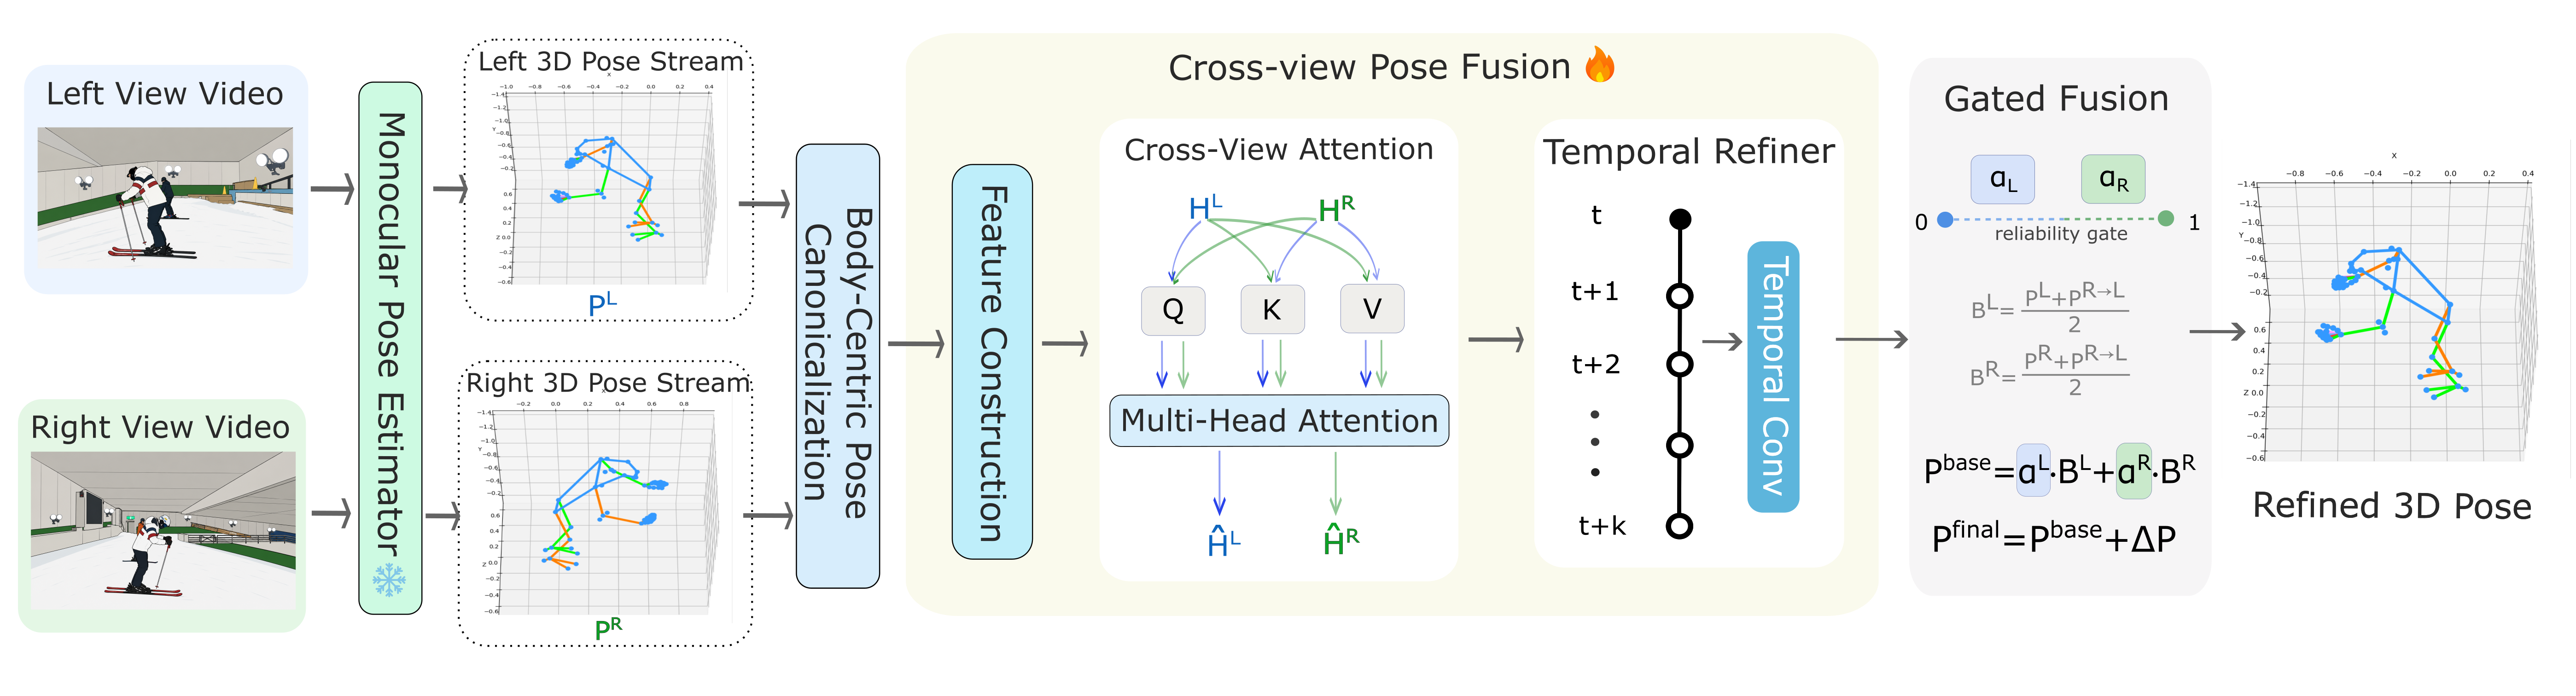
\includegraphics[width=\textwidth]{figure/intro1.png}
  \caption{Overview of the proposed calibration-free dual-view 3D pose refinement framework.}
  \Description{Overview of the proposed dual-view 3D pose refinement framework, from body-centric canonicalization and cross-view alignment to attention-based feature exchange, temporal refinement, reliability-gated fusion, and residual correction.}
  \label{fig:teaser}
\end{teaserfigure}

% \received{TODO}
% \received[revised]{TODO}
% \received[accepted]{TODO}

%%
%% This command processes the author and affiliation and title
%% information and builds the first part of the formatted document.
\maketitle

\section{Introduction}

Accurate 3D human pose estimation is a fundamental component of sports motion analysis, with applications in performance evaluation, skill assessment, injury prevention, and coaching support. In skiing and other fast outdoor sports, however, recovering reliable 3D body motion remains challenging. Athletes move rapidly, body parts are frequently self-occluded, and viewpoints change with respect to the skier's body orientation. These factors often lead to depth ambiguity, unstable limb predictions, and frame-wise jitter when 3D pose is estimated from a single camera view.

Multi-view capture can reduce these ambiguities by observing the athlete from complementary viewpoints. A common solution is to calibrate all cameras and reconstruct 3D pose through geometric triangulation or calibrated multi-view learning. While effective in controlled environments, such requirements are restrictive in practical sports recording. Cameras may be temporarily installed on slopes, handheld or mounted at different positions, and difficult to calibrate accurately before every session. In addition, field videos are often processed by existing monocular 3D pose estimators, producing independent pose streams for each view rather than raw multi-view keypoints with known camera parameters. This creates a practical but less studied problem: how to refine and fuse two already-estimated 3D pose sequences when full camera calibration is unavailable.

This paper addresses calibration-free post-estimation dual-view 3D pose refinement for sports motion analysis. In this work, \textit{calibration-free} means that the refinement model does not take camera intrinsics, camera extrinsics, epipolar geometry, or triangulated image observations as input at training or inference time. The method assumes only synchronized left- and right-view 3D pose streams produced by an upstream monocular estimator. Dataset preparation and evaluation may still use synchronized recordings or dataset-provided references; these are not supplied to the refinement network. Under this setting, the proposed framework operates directly on left- and right-view 3D pose streams. The input poses are first transformed into a body-centric canonical coordinate representation to reduce global differences in position, orientation, and scale. We then perform pose-level cross-view alignment to construct aligned opposite-view poses and residual disagreement features. These features allow the network to reason about where the two views agree, where they conflict, and which view may provide more reliable evidence for a particular joint and frame.

To exploit the complementary information between views, the framework encodes geometric and motion cues for each joint and applies bidirectional cross-view attention. The attended features are further processed by a temporal refinement module to improve motion continuity and suppress jitter. Finally, a reliability-gated fusion module predicts joint-frame view weights and combines the two pose candidates with a residual correction. This design differs from simple averaging: rather than assuming that both views are equally reliable everywhere, the model learns to adapt fusion according to cross-view disagreement and temporal context.

We evaluate the proposed method on two skiing datasets with complementary evidence. The Unity synthetic dataset provides recorded avatar skeletons and supports evaluation against available 3D ground truth. The real-world Ski-PTZ-Pose dataset provides synchronized skiing views and dataset annotations, but in our setting it is evaluated against a fused canonical reference pose rather than an independent physical ground-truth capture. The experiments compare the proposed model with single-view inputs and simple fusion baselines using pose accuracy and temporal stability metrics, and we explicitly interpret Ski-PTZ-Pose results as fused-reference agreement. We further conduct masking robustness experiments to simulate missing or unreliable pose inputs caused by occlusion, tracking failure, or upstream pose-estimation errors.

The main contributions of this work are threefold:
\begin{itemize}
    \item We formulate a calibration-free post-estimation dual-view 3D pose refinement problem for sports motion analysis, where two independently estimated 3D pose streams are refined without relying on full camera calibration.
    
    \item We propose a cross-view refinement framework that combines body-centric canonicalization, pose-level alignment, bidirectional cross-view attention, temporal refinement, reliability-gated fusion, and residual correction to produce more accurate and temporally stable 3D pose sequences.
    \item We evaluate the proposed method on a Unity synthetic skiing dataset with recorded avatar skeletons and on the real-world Ski-PTZ-Pose dataset using a fused canonical reference, reporting the latter as reference-agreement rather than independent physical ground-truth accuracy.
\end{itemize}

\section{Related Work}
\label{sec:related_work}

\subsection{Monocular 3D Human Pose Estimation}
Monocular 3D human pose estimation has progressed from temporal convolutional lifting models to transformer-based architectures and large-scale motion representation learning. VideoPose3D introduced temporal convolutional modeling for lifting 2D keypoint sequences to 3D poses, while PoseFormer and MHFormer employed transformer architectures and multi-hypothesis representations to capture long-range temporal dependencies and reduce depth ambiguity. Large-scale motion representation learning, such as MotionBERT, further improves generalization across human-centric motion tasks~\cite{pavllo2019videopose3d,zheng2021poseformer,li2022mhformer,zhu2023motionbert}. Single-image foundation-model-based approaches such as SAM 3D Body further enable robust monocular full-body pose and shape estimation from in-the-wild images, making it practical to obtain per-frame 3D pose streams from field videos~\cite{yang2026sam}. Related video-based human modeling approaches such as VIBE also demonstrate the importance of temporal priors for stabilizing human motion estimation in unconstrained environments~\cite{kocabas2020vibe}. Despite these advances, existing monocular approaches estimate each video stream independently and primarily focus on improving pose quality within a single viewpoint. Consequently, depth ambiguity, self-occlusion, and viewpoint-dependent errors remain challenging, particularly in fast sports motions such as skiing. However, these methods do not explicitly exploit complementary information available across synchronized viewpoints.

% Monocular 3D human pose estimation has advanced from frame-wise lifting to video-based temporal modeling. Temporal convolutional models, transformer-based approaches, and motion representation learning improve robustness by exploiting spatial and temporal context~\cite{pavllo2019videopose3d,zheng2021poseformer,li2022mhformer,zhu2023motionbert}. These methods are effective for monocular sequences, but depth ambiguity, self-occlusion, and viewpoint-dependent errors remain problematic in fast sports motion. Sports-oriented work such as the Ski-Pose PTZ-Camera dataset demonstrates the importance and difficulty of estimating 3D pose in real skiing scenes with large body motion and changing viewpoints~\cite{rhodin2018learning}. Video-based body models further show that temporal priors are important for stabilizing in-the-wild human motion~\cite{kocabas2020vibe}.

\subsection{Multi-view 3D Human Pose Estimation}
Multi-view pose estimation reduces monocular ambiguity by triangulating detections, aggregating cross-view evidence, or learning geometry-aware feature fusion across synchronized camera views. Representative approaches include Learnable Triangulation~\cite{iskakov2019learnable}, which incorporates differentiable triangulation into end-to-end learning, and Epipolar Transformers~\cite{he2020epipolar}, which exploit epipolar geometry for cross-view feature aggregation. More recent geometry-aware transformer frameworks, such as Geometry-Biased Transformer (GBT) and MVGFormer, further improve multi-view reconstruction by incorporating geometric constraints into attention mechanisms and cross-view feature interaction~\cite{venkat2023geometry,liao2024multiple}. However, these approaches typically require known camera calibration and synchronized multi-view observations, making their deployment more challenging in practical sports recordings where accurate camera parameters may be unavailable and only estimated pose streams are accessible. Recent efforts have also explored uncalibrated or weakly calibrated settings. MetaPose learns multi-view 3D pose without direct 3D supervision, and FLEX estimates human motion without known extrinsic parameters~\cite{usman2022metapose,gordon2022flex}. Despite relaxing calibration requirements, these methods still estimate 3D pose or motion jointly from synchronized multi-view observations, such as images, videos, or 2D keypoint detections, and remain tightly coupled to the multi-view pose reconstruction process. In contrast, our work targets a complementary post-estimation setting: given independently estimated dual-view pose streams, we refine them directly in pose space by enforcing cross-view and temporal consistency. This design avoids the need for camera calibration or image-level reconstruction, while leveraging cross-view and temporal cues to reduce disagreement and temporal jitter between pose streams.
% Multi-view pose estimation can reduce monocular ambiguity by triangulating detections or exchanging features across views. Learnable triangulation and epipolar-transformer methods exploit calibrated camera geometry to improve reconstruction accuracy~\cite{iskakov2019learnable,he2020epipolar}. Such approaches are well suited to laboratory or studio capture, where camera intrinsics, extrinsics, and synchronized image observations can be controlled. In sports recording, however, cameras may be temporarily installed, handheld, or moved between sessions, making repeated calibration costly and error-prone. This creates a gap between calibrated multi-view reconstruction and practical field analysis, where the available data are often already-estimated pose tracks rather than raw calibrated multi-view detections.

% Weakly calibrated and calibration-free multi-view methods reduce the dependence on full camera parameters. MetaPose learns multi-view 3D pose without direct 3D supervision, and FLEX estimates human motion without known extrinsic parameters~\cite{usman2022metapose,gordon2022flex}. These methods address an important relaxation of camera requirements, but they still primarily operate at the image, 2D keypoint, or multi-view reconstruction stage. In contrast, our target setting is post-estimation refinement: two monocular 3D pose sequences are already available, and the goal is to improve their accuracy and temporal stability without revisiting image-level reconstruction or estimating camera geometry.

Collectively, existing methods focus either on improving monocular pose estimation or reconstructing poses jointly from multiple views. Our work instead considers calibration-free post-estimation refinement of independently estimated dual-view pose streams. By canonicalizing poses into a shared body-centric representation, aligning them at the pose level, and learning joint-frame reliability for fusion, the proposed framework exploits cross-view consistency to reduce disagreement and temporal jitter using only pose-space information.

\section{Proposed Method}
\label{sec:method}

\subsection{Overview}
\label{subsec:method_overview}

Figure~\ref{fig:teaser} gives an overview of the proposed calibration-free dual-view 3D pose refinement framework for sports motion analysis. The method takes two independently estimated 3D pose sequences as input and predicts a refined 3D pose sequence. Unlike calibrated multi-view reconstruction methods, the proposed framework does not assume full camera intrinsic or extrinsic parameters. Instead, it operates directly on two 3D pose streams and refines them in a canonical pose space.

Let \(P^L, P^R \in \mathbb{R}^{T \times J \times 3}\) denote the left-view and right-view 3D pose sequences, where \(T\) is the number of frames and \(J\) is the number of joints. The goal is to estimate a refined pose sequence \(P^F \in \mathbb{R}^{T \times J \times 3}\) that is more accurate and temporally stable than either input stream or simple average fusion.

The overall framework consists of five main stages. First, both input pose streams are transformed into a body-centric canonical coordinate representation. Second, pose-level cross-view alignment is used to construct aligned opposite-view poses and cross-view residual features. Third, geometric and motion features are encoded by a joint-wise encoder and exchanged through bidirectional cross-view attention. Fourth, a temporal refinement module models local motion continuity along the time dimension. Finally, the model predicts a joint-frame reliability gate and a residual pose correction to produce the refined output.

\subsection{Body-Centric Pose Canonicalization}
\label{subsec:canonicalization}

The two input pose streams may differ in global position, orientation, and scale because they are estimated independently from different camera views. Directly averaging them can therefore be unreliable. To reduce this discrepancy, we first transform each pose sequence into a body-centric canonical coordinate system.

Given an input pose sequence \(P\), we define a canonicalization function \(\mathcal{C}(\cdot)\) using stable body landmarks, including the left hip, right hip, and neck. For each frame, the pelvis center is used as the origin, the hip-to-hip direction defines the lateral body axis, and the pelvis-to-neck direction defines the torso direction. These axes are orthonormalized to construct a body-centric rotation. The pose is translated to the pelvis origin, rotated into this body-centric frame, and normalized by a skeleton scale computed from stable torso and hip distances. The left and right pose streams are transformed as
\[
\tilde{P}^{L} = \mathcal{C}(P^L), 
\qquad
\tilde{P}^{R} = \mathcal{C}(P^R),
\]
where \(\tilde{P}^{L}\) and \(\tilde{P}^{R}\) denote the canonicalized left-view and right-view pose sequences.

This canonicalization is not intended to estimate physical camera geometry. Instead, it provides a shared normalized pose representation that makes the two independently estimated 3D pose streams comparable before cross-view refinement. The output of the refinement model is also represented in this canonical pose space.

\subsection{Pose-Level Cross-View Alignment}
\label{subsec:pose_alignment}

Although body-centric canonicalization reduces global pose differences, residual misalignment may remain between the two pose streams. We therefore apply pose-level cross-view alignment in both directions. Specifically, the left pose sequence is aligned to the right pose sequence, and the right pose sequence is aligned to the left pose sequence:
\[
\tilde{P}^{L \rightarrow R} = \mathcal{A}(\tilde{P}^{L}, \tilde{P}^{R}),
\qquad
\tilde{P}^{R \rightarrow L} = \mathcal{A}(\tilde{P}^{R}, \tilde{P}^{L}),
\]
where \(\mathcal{A}(\cdot)\) denotes sequence-level pose alignment.

In implementation, the alignment is computed over all joints and frames in the sequence by solving a similarity alignment between the two canonicalized pose streams. The same sequence-level transform is applied to every joint and frame in the source stream, producing an aligned auxiliary pose and a compact rotation cue for feature construction. The resulting aligned poses are used only as pose-level auxiliary representations. They should not be interpreted as calibrated camera transformations. This design allows the model to exploit cross-view geometric consistency without requiring full camera calibration.

We further compute cross-view residuals:
\[
D^{L} = \tilde{P}^{R \rightarrow L} - \tilde{P}^{L},
\qquad
D^{R} = \tilde{P}^{L \rightarrow R} - \tilde{P}^{R}.
\]
These residuals encode disagreement between the two pose streams and provide cues about view-specific errors.

\subsection{Geometric-Motion Feature Construction}
\label{subsec:feature_construction}

\begin{figure}
  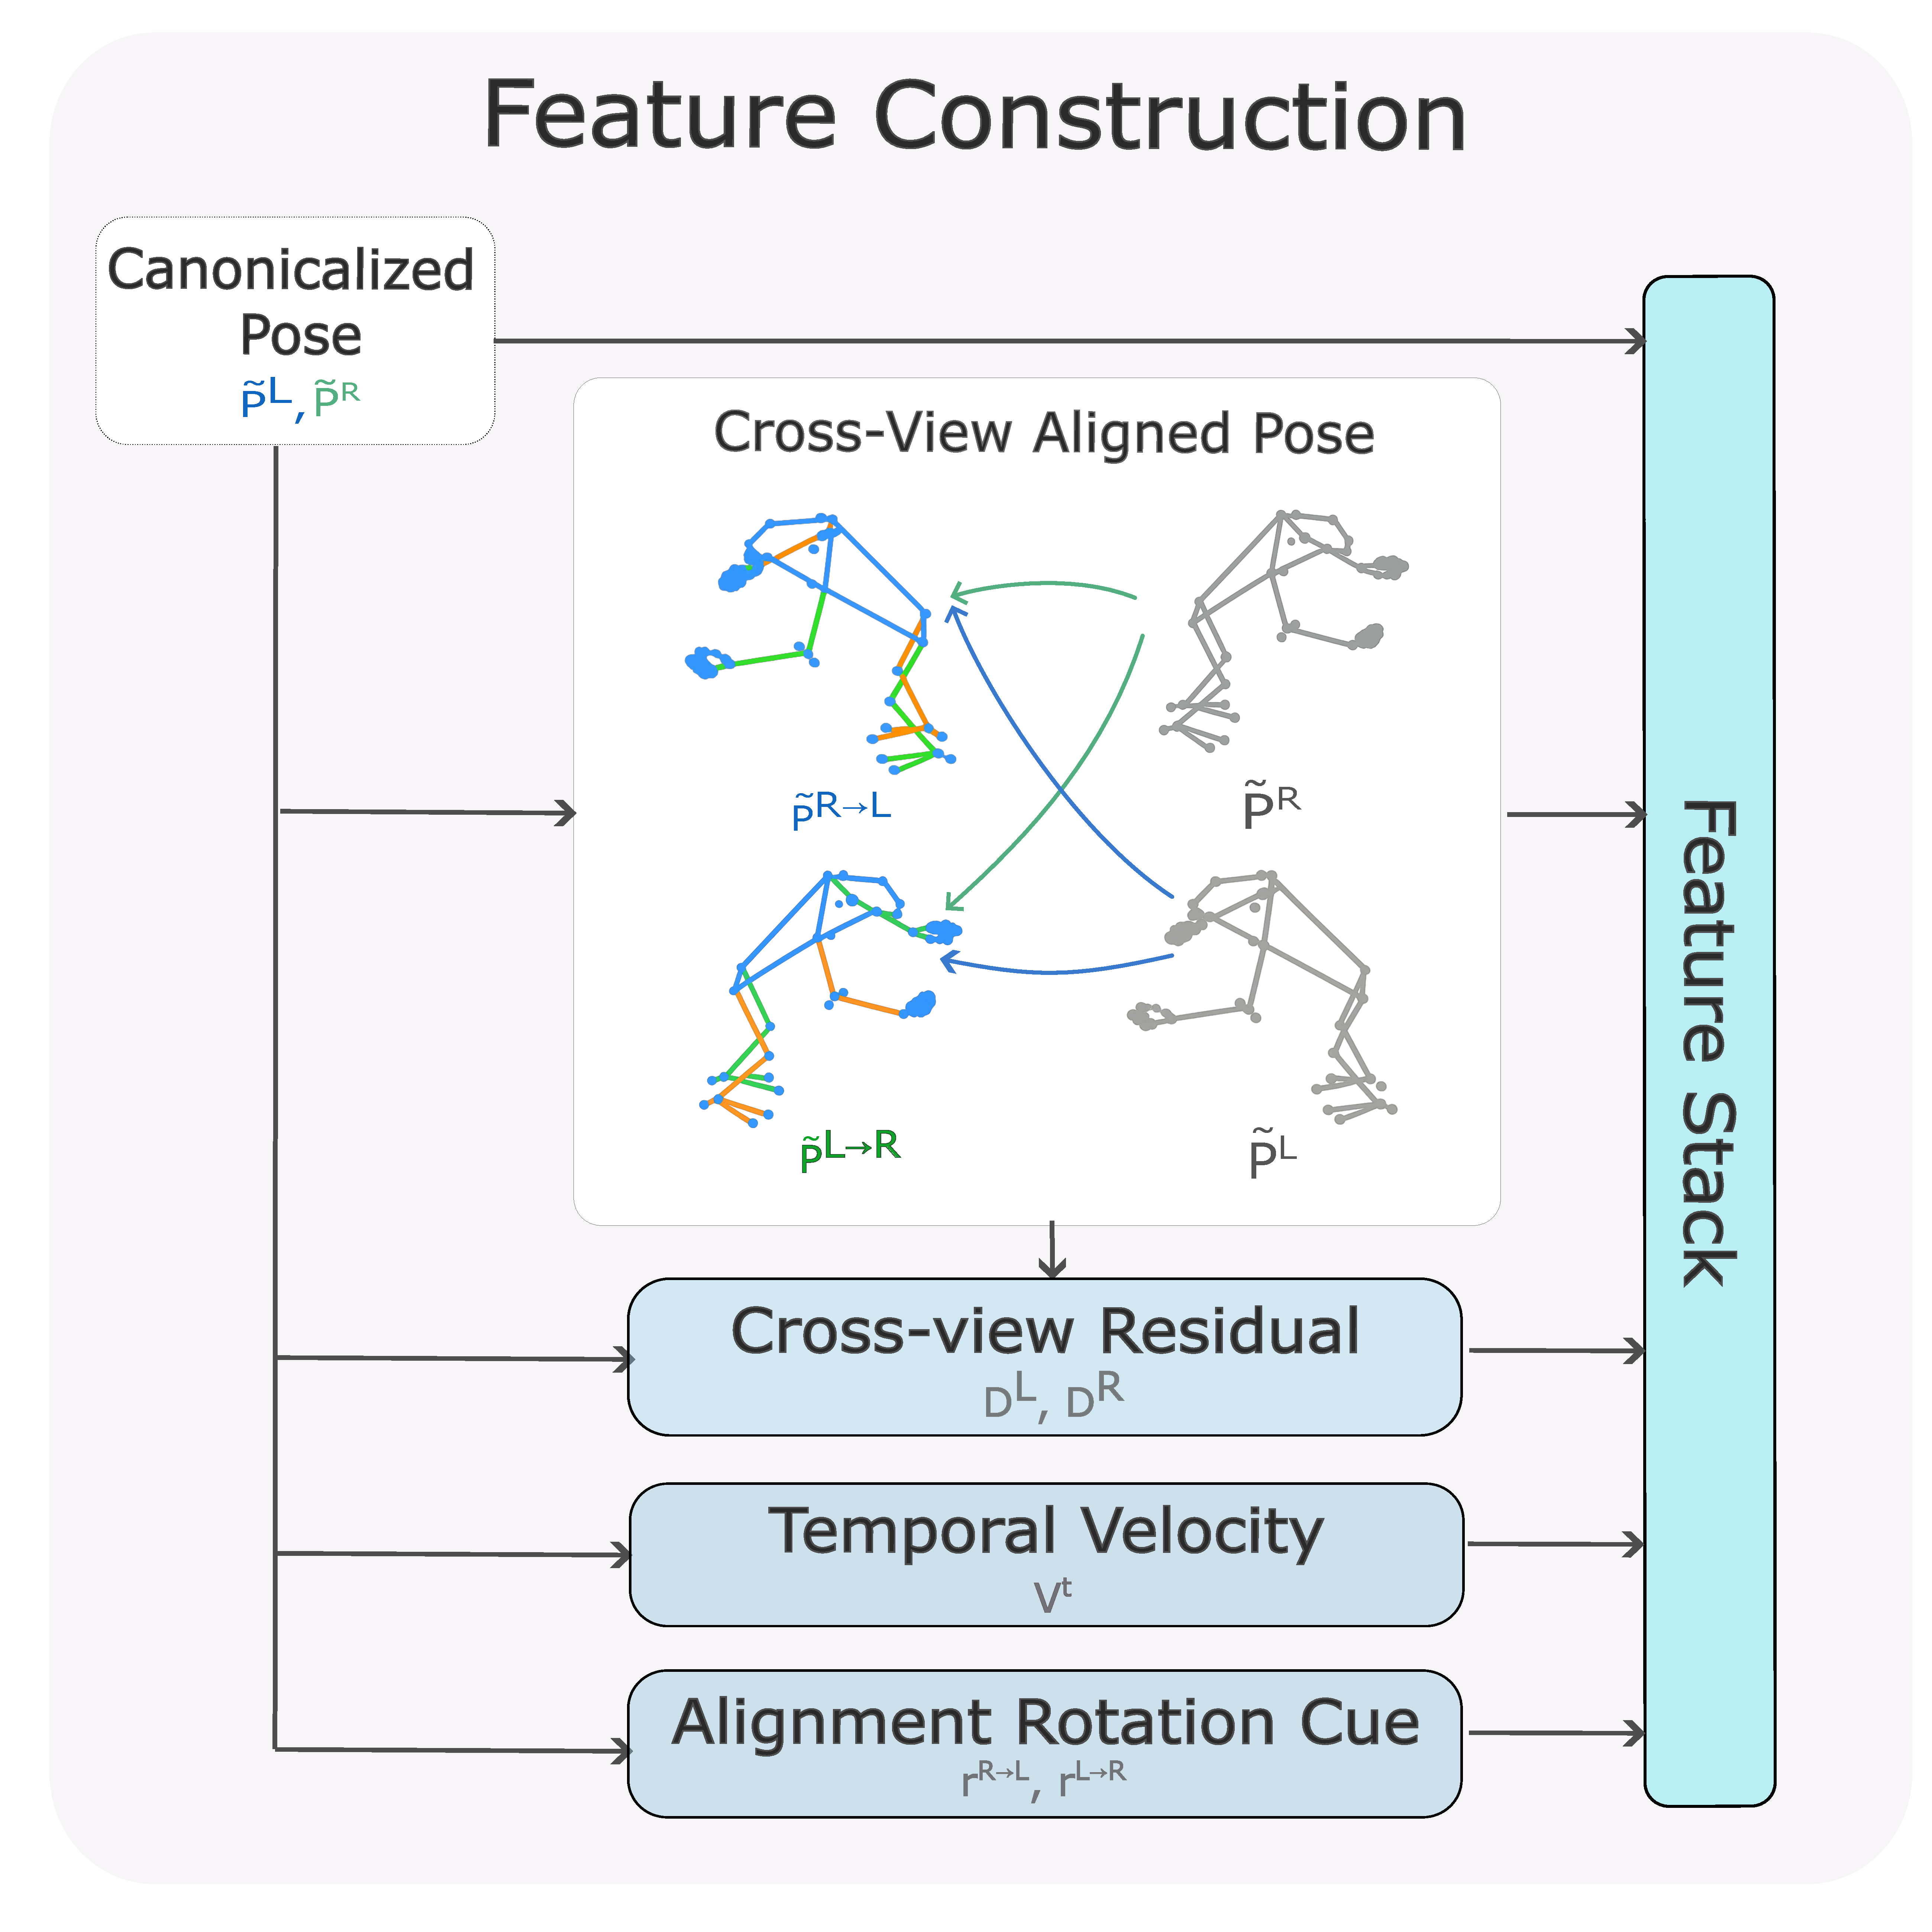
\includegraphics[width=0.8\linewidth]{figure/fig2.pdf}
  \caption{Geometric-motion feature construction for dual-view pose refinement.}
  \Description{Diagram showing how each view combines its canonical pose, the aligned opposite-view pose, residual disagreement, velocity, and rotation cues into joint-level geometric-motion features.}
  \label{fig:feature_construction}
\end{figure}

As shown in Figure~\ref{fig:feature_construction}, for each view, we construct joint-level geometric-motion features by concatenating pose, cross-view, and temporal cues. For the left-view stream, the feature is defined as
\[
X^{L}
=
\left[
\tilde{P}^{L},
\tilde{P}^{R \rightarrow L},
D^{L},
V^{L},
r^{R \rightarrow L}
\right],
\]
and for the right-view stream,
\[
X^{R}
=
\left[
\tilde{P}^{R},
\tilde{P}^{L \rightarrow R},
D^{R},
V^{R},
r^{L \rightarrow R}
\right].
\]

Here, \(V^{L}\) and \(V^{R}\) denote frame-to-frame velocity features computed from the canonical pose sequences, with the first-frame velocity set to zero. The terms \(r^{R \rightarrow L}\) and \(r^{L \rightarrow R}\) denote 3D rotation-vector cues derived from the pose-level alignment in each direction and broadcast to all joints and frames in the corresponding sequence. Each component is represented in 3D, resulting in a 15-dimensional feature vector for each joint at each frame.

This feature design provides the network with four types of information: the view's own pose estimate, the opposite view aligned into the same pose space, the residual disagreement between views, and local motion cues. These cues are useful for deciding which view should be trusted for each joint and frame.

\subsection{Joint Feature Encoding}
\label{subsec:joint_feature_encoding}

The left and right geometric-motion features are passed through a shared joint-wise encoder:
\[
H^{L} = \phi(X^{L}),
\qquad
H^{R} = \phi(X^{R}),
\]
where \(\phi(\cdot)\) is a multilayer perceptron with layer normalization and GELU activation. The encoder maps the 15-dimensional input feature into a hidden representation for each joint and frame.

Because the encoder is applied at the joint-feature level, it preserves the temporal and skeletal structure of the input sequence while producing a richer representation for subsequent cross-view interaction.

\subsection{Bidirectional Cross-View Attention}
\label{subsec:cross_view_attention}

To exchange complementary information between the two pose streams, we use bidirectional cross-view attention. For each frame, the left-view joint features attend to the right-view joint features, and the right-view joint features attend to the left-view joint features:
\[
\hat{H}^{L}
=
\mathrm{Attn}(Q=H^{L}, K=H^{R}, V=H^{R}),
\]
\[
\hat{H}^{R}
=
\mathrm{Attn}(Q=H^{R}, K=H^{L}, V=H^{L}).
\]

The attention is applied over joints within each frame. This allows the network to compare corresponding and related joint features across the two views. When a joint is unreliable in one view, the other view may provide complementary information. Residual connections and layer normalization are used to stabilize the cross-view feature update.

\subsection{Temporal Refinement}
\label{subsec:temporal_refinement}

Sports motion contains strong temporal structure. Frame-wise fusion alone may reduce spatial error but can still produce temporally unstable pose trajectories. To address this issue, we apply a temporal refinement module after cross-view attention.

The temporal refiner uses depthwise one-dimensional convolution along the time dimension. For each joint, the hidden feature sequence is normalized and passed through a temporal convolution block:
\[
\bar{H} = \hat{H} + \mathrm{TempConv}(\mathrm{LN}(\hat{H})).
\]
This residual formulation preserves the original cross-view representation while adding local temporal context. The temporal module is lightweight and targets short-range motion consistency, which is important for reducing jitter in sports pose sequences.

\subsection{Reliability-Gated Fusion and Residual Correction}
\label{subsec:reliability_fusion}

After cross-view attention and temporal refinement, the left and right hidden features are concatenated:
\[
Z = [\bar{H}^{L}, \bar{H}^{R}].
\]
A gate head predicts a joint-frame reliability gate:
\[
\alpha = \sigma(g_{\theta}(Z)),
\]
where \(\alpha \in [0,1]^{T \times J \times 1}\). The gate controls the relative contribution of the two view-specific pose candidates for each joint and frame.

All pose candidates used in the fusion step are represented in the same body-centric canonical pose space. The alignment directions \(R \rightarrow L\) and \(L \rightarrow R\) indicate how the auxiliary opposite-view poses are constructed, but they do not define separate physical camera coordinate frames. After alignment, both base candidates are interpreted in a single canonical fusion frame defined by the body-centric normalization, rather than in two camera-specific coordinate systems. Thus, the two base candidates below can be combined by the reliability gate in this shared canonical frame.

We construct two base pose candidates:
\[
B^{L} = \frac{1}{2}(\tilde{P}^{L} + \tilde{P}^{R \rightarrow L}),
\]
\[
B^{R} = \frac{1}{2}(\tilde{P}^{R} + \tilde{P}^{L \rightarrow R}).
\]
The reliability-gated base fusion is then computed as
\[
P^{base}
=
\alpha B^{L}
+
(1-\alpha)B^{R}.
\]

Finally, a residual head predicts a pose correction:
\[
\Delta P = h_{\theta}(Z),
\]
and the final refined pose is
\[
P^{F} = P^{base} + \Delta P.
\]

The gate \(\alpha\) is interpreted as a learned reliability signal rather than a calibrated probabilistic uncertainty estimate. This distinction is important because the model is trained to improve fusion accuracy and temporal stability, not to produce calibrated uncertainty values.

\subsection{Training Objective}
\label{subsec:training_objective}

The model is trained with a supervised pose loss and lightweight regularization terms:
\[
\mathcal{L}
=
\mathcal{L}_{sup}
+
\lambda_{view}\mathcal{L}_{view}
+
\lambda_{bal}\mathcal{L}_{bal}
+
\lambda_{ent}\mathcal{L}_{ent}
+
\lambda_{temp}\mathcal{L}_{temp}.
\]
The supervised term is \(\mathcal{L}_{sup}=\|P^{F}-\tilde{G}\|_{1}\), where \(\tilde{G}\) denotes the canonicalized reference pose. For Unity, \(\tilde{G}\) is obtained from the recorded avatar skeleton; for Ski-PTZ-Pose, it is the fused canonical reference pose described in Section~\ref{subsec:dataset_annotation}. Therefore, Ski-PTZ-Pose supervision and evaluation measure agreement with this canonical reference rather than accuracy against independent motion-capture-style ground truth. The view reconstruction term preserves information from both input streams using aligned residuals rather than raw cross-view differences. We define \(\delta^{L}=\tilde{P}^{L}-\tilde{P}^{R\rightarrow L}\) and \(\delta^{R}=\tilde{P}^{R}-\tilde{P}^{L\rightarrow R}\), and reconstruct \(\hat{P}^{L}=P^{F}+(1-\alpha)\delta^{L}\) and \(\hat{P}^{R}=P^{F}-\alpha\delta^{R}\). The reconstruction loss penalizes their \(L_{1}\) errors to \(\tilde{P}^{L}\) and \(\tilde{P}^{R}\), respectively. To avoid degenerate fusion, \(\mathcal{L}_{bal}=|\mathrm{mean}(\alpha)-0.5|\) discourages collapse to a single view, while an entropy term discourages overconfident gates during training. Finally, \(\mathcal{L}_{temp}\) penalizes excessive second-order temporal variation of \(P^{F}\), encouraging stable motion trajectories without removing the supervised accuracy objective.

\section{Experiments}

\subsection{Experimental Setup}

We evaluate a calibration-free post-estimation setting. For each sequence, left- and right-view videos are first processed independently by the same upstream monocular 3D pose estimator, producing two noisy 3D pose streams. The proposed model and all fusion baselines then operate only on these pose sequences; camera intrinsics and extrinsics are not used as model inputs. For fair comparison, predictions and reference poses are mapped to a common joint subset and evaluated in the same body-centric canonical pose space. Unity results are measured against the recorded avatar skeleton, whereas Ski-PTZ-Pose results are measured as agreement with the fused canonical reference. We compare against single-view predictions and simple fusion baselines, including raw averaging and pseudo canonical fusion.

\subsection{Datasets and Annotation}
\label{subsec:dataset_annotation}

We use two complementary skiing datasets: a Unity synthetic dataset collected for controlled evaluation and the public Ski-Pose PTZ-Camera dataset, denoted as \textit{Ski-PTZ-Pose}, for real-world alpine skiing evaluation. Unity provides synchronized dual-view sequences with directly available 3D avatar skeletons, whereas Ski-PTZ-Pose provides real skiing videos, 3D skier poses, projected 2D poses, and PTZ-camera calibration from EPFL/CVLab~\cite{ski_poseptz_dataset}. The proposed refinement model does not use the PTZ calibration parameters as input. They are part of the dataset metadata and are used only to interpret the dataset-provided annotations and construct evaluation references. Table~\ref{tab:dataset_summary} summarizes the roles of the two datasets.

\begin{table*}[t]
\centering
\caption{Summary of the datasets used in this study.}
\label{tab:dataset_summary}
\footnotesize
\setlength{\tabcolsep}{2pt}
\renewcommand{\arraystretch}{1.05}
\begin{tabular}{@{}>{\raggedright\arraybackslash}p{0.22\linewidth}
                >{\raggedright\arraybackslash}p{0.16\linewidth}
                >{\raggedright\arraybackslash}p{0.28\linewidth}
                >{\raggedright\arraybackslash}p{0.24\linewidth}@{}}
\hline
Dataset & Source & Item & Role / Reference \\
\hline
\multirow{2}{*}{Unity synthetic}
& \multirow{2}{*}{Ours}
& Dual-view videos and monocular 3D poses
& Training / testing inputs \\
& & Avatar 3D skeleton
& 15-joint GT; robustness \\
\hline
\multirow{2}{*}{Ski-PTZ-Pose}
& \multirow{2}{*}{EPFL/CVLab}
& Real skiing videos and 2D/3D poses
& Real-world evaluation \\
& & PTZ metadata
& Fused canonical reference only \\
\hline
\end{tabular}
\end{table*}

\paragraph{Unity synthetic dataset.}
We rendered a virtual skiing scene from two synchronized cameras that mimic left and right sports-recording viewpoints. Two avatar characters perform six skiing-related actions: Braking, Fall, Idle, Losing, Straight, and Winning. The rendered videos are processed by the upstream monocular estimator to obtain left- and right-view 3D pose streams, while ground-truth 3D joints are recorded from the Unity skeleton and mapped to a common 15-joint subset.

\paragraph{Ski-Pose PTZ-Camera dataset.}
Ski-PTZ-Pose contains competitive alpine skiers performing giant slalom runs captured by multiple pan-tilt-zoom cameras~\cite{rhodin2018learning}. It provides 22 human joints and projected 2D poses for each camera view in approximately 20K images, together with per-frame PTZ-camera calibration. In our experiments, the calibration parameters are not used by the refinement model. Since the available 3D annotations are view-specific rather than a single motion-capture-style world skeleton, we construct a \textit{fused reference pose} for evaluation by synchronizing views at the same timestamp, mapping the available joints to the common 15-joint subset, canonicalizing each view-specific 3D pose, and averaging the canonicalized references. This fused reference is used only for metric computation and should be interpreted as an evaluation reference rather than an independent physical ground-truth capture. We therefore report Ski-PTZ-Pose errors in canonical reference space.

\subsection{Implementation Details}
\label{subsec:implementation_details}

All methods operate on the same synchronized left- and right-view pose windows after mapping the upstream predictions to the common 15-joint skeleton. The input to the proposed model is a tensor of joint-frame pose features in canonical space; no RGB frames, 2D keypoints, masks, camera intrinsics, or camera extrinsics are provided to the refinement network. Left and right streams are canonicalized independently and then aligned in both directions to form the auxiliary opposite-view poses and residual features described in Section~\ref{sec:method}.

The joint-wise encoder is implemented as a shared multilayer perceptron applied to each joint-frame feature vector. Cross-view attention is applied within each frame over the joint dimension, allowing each view to attend to the corresponding and anatomically related joints in the opposite view. The temporal refiner is a lightweight depthwise one-dimensional convolution over time, applied independently for each joint feature trajectory. The gate and residual heads are linear prediction heads on the concatenated left and right hidden features. The gate output is constrained by a sigmoid and predicts one scalar reliability weight per joint and frame.

During training, the supervised target is the canonicalized reference pose: the Unity avatar skeleton for the synthetic dataset and the fused canonical reference pose for Ski-PTZ-Pose. Thus, Ski-PTZ-Pose training targets the constructed canonical reference rather than independent physical ground truth. All reported experiments use 30-frame input windows, a hidden dimension of 128, four cross-view attention heads, and a temporal convolution kernel size of 3. The model is optimized with AdamW using a learning rate of \(1.0 \times 10^{-3}\), a batch size of 64, and 200 training epochs. The loss weights \(\lambda_{view}\), \(\lambda_{bal}\), \(\lambda_{ent}\), and \(\lambda_{temp}\) are set to 0.1, 0.01, 0.001, and 0.01, respectively. We split each dataset by sequence into 70\% training, 15\% validation, and 15\% test sets, and use a fixed random seed of 42 for all experiments.

For fair comparison, all baselines use the same input pose streams, joint subset, synchronization, canonicalization, and evaluation protocol as the proposed model. Raw-space baselines are reported separately to show the magnitude of unnormalized upstream prediction errors, but the main comparisons are the canonical-space methods.

\subsection{Evaluation Metrics and Robustness Protocol}

We report two metrics. \textbf{MPJPE} measures the mean Euclidean distance between predicted and reference 3D joints over all frames and joints. For Unity, the reference is the directly recorded avatar skeleton; for Ski-PTZ-Pose, it is the fused canonical reference described above, so the metric reports canonical-reference agreement. \textbf{Acceleration error} compares the second-order finite differences \(P_{t+1,j}-2P_{t,j}+P_{t-1,j}\) of predicted and reference sequences, measuring temporal motion consistency in the same canonical space. Lower values are better for both metrics.

To evaluate robustness, we mask the input 3D pose streams to simulate missing or unreliable joints caused by occlusion, tracking failure, or upstream pose-estimation errors. We test three masking protocols. Random joint-frame masking independently removes sampled joints at individual frames. Distal-joint masking corrupts limb-end joints such as wrists and ankles, which are frequently unreliable in skiing motion. Temporal masking removes contiguous short frame intervals to simulate burst occlusion or tracking failure. We compare the proposed model with canonical average fusion under the same corrupted inputs.

\section{Results and Discussion}

\subsection{Overall Pose Accuracy}

Table~\ref{tab:accuracy_temporal_combined} shows that the proposed model improves over single-view inputs and simple fusion baselines under the current evaluation protocol. Compared with pseudo canonical fusion, MPJPE decreases from \(0.3705\) to \(0.2711\) on Unity against the recorded avatar skeleton. On Ski-PTZ-Pose, MPJPE decreases from \(0.3487\) to \(0.1794\), which should be interpreted as improved agreement with the fused canonical reference rather than independent physical 3D ground-truth accuracy. The model also achieves the lowest acceleration error in the same canonical evaluation space.

The gap between raw-space and canonical-space baselines indicates that representation normalization is a necessary first step but is not sufficient by itself. Canonical average fusion reduces view-dependent scale and orientation variation, yet it still treats the two pose streams as equally reliable at every joint and frame. The proposed model improves beyond this baseline because it can use cross-view correspondence, temporal context, and residual correction to make local decisions. This behavior is important for skiing motions, where distal joints and asymmetric body turns often make one view temporarily more informative than the other.

\begin{table*}[t]
\centering
\caption{Accuracy and temporal stability on Unity and Ski-PTZ-Pose. Lower values are better; canonical-space methods provide the main comparison.}
\label{tab:accuracy_temporal_combined}
\setlength{\tabcolsep}{6pt}
\renewcommand{\arraystretch}{1.12}
\begin{tabular}{lcccc}
\hline
\multirow{2}{*}{Method} &
\multicolumn{2}{c}{Unity} &
\multicolumn{2}{c}{Ski-PTZ-Pose} \\
\cline{2-5}
& MPJPE \(\downarrow\) & Accel. Err. \(\downarrow\)
& MPJPE \(\downarrow\) & Accel. Err. \(\downarrow\) \\
\hline
Left raw SAM3D
& 2.0536 & 0.0430
& 1.0962 & 0.0543 \\

Right raw SAM3D
& 2.0541 & 0.0441
& 1.0112 & 0.0454 \\

Naive raw fusion
& 2.0349 & 0.0360
& 1.0170 & 0.0397 \\
\hline
Left canonical
& 0.4161 & 0.0401
& 0.3552 & 0.0531 \\

Right canonical
& 0.4202 & 0.0402
& 0.4462 & 0.0455 \\

Pseudo canonical fusion
& 0.3705 & 0.0326
& 0.3487 & 0.0392 \\

Proposed model
& \textbf{0.2711} & \textbf{0.0312}
& \textbf{0.1794} & \textbf{0.0311} \\
\hline
\end{tabular}
\vspace{0.5em}
\begin{minipage}{0.95\linewidth}
\footnotesize
\textit{Note.} Acceleration error measures the discrepancy between predicted and reference second-order temporal motion. Raw-space and canonical-space values should not be interpreted as a direct comparison because canonicalization changes the pose representation.
\end{minipage}

\end{table*}

To examine whether the learned gate collapses to a single view or preserves local fusion flexibility, we summarize the predicted fusion weights in Table~\ref{tab:gate_region_summary}. The reported value is the mean left-candidate weight \(\alpha\), averaged over frames and joints within each body region; \(1-\alpha\) is the corresponding right-candidate weight. The learned gates remain close to balanced on average, which is consistent with the balance regularization in the training objective, while still showing small region-dependent variations. This suggests that the model does not simply select one pose stream globally, but retains joint-level flexibility after cross-view alignment and temporal refinement.

\begin{table}[t]
\centering
\caption{Region-wise reliability-gate statistics under representative evaluation settings. \(\alpha\) denotes the learned left-candidate fusion weight, and \(1-\alpha\) denotes the right-candidate weight.}
\label{tab:gate_region_summary}
\footnotesize
\setlength{\tabcolsep}{4.2pt}
\renewcommand{\arraystretch}{1.08}
\begin{tabular}{llccc}
\hline
Dataset & Region & Joints & \(\alpha\) & \(1-\alpha\) \\
\hline
\multirow{3}{*}{Unity}
& Upper limbs & 6 & \(0.497 \pm 0.004\) & 0.503 \\
& Lower limbs & 6 & \(0.502 \pm 0.014\) & 0.498 \\
& All joints & 15 & \(0.497 \pm 0.011\) & 0.503 \\
\hline
\multirow{3}{*}{Ski-PTZ}
& Upper limbs & 6 & \(0.522 \pm 0.005\) & 0.478 \\
& Lower limbs & 6 & \(0.491 \pm 0.018\) & 0.509 \\
& All joints & 13 & \(0.508 \pm 0.020\) & 0.492 \\
\hline
\end{tabular}
\vspace{0.4em}
\begin{minipage}{0.95\linewidth}
\footnotesize
\textit{Note.} Values report the mean and across-joint standard deviation of per-joint mean \(\alpha\) within each region. Statistics are computed from exported gate summaries on the Unity no-mask setting and the available Ski-PTZ random-mask evaluation setting. The gate is a learned fusion signal, not a calibrated uncertainty estimate.
\end{minipage}
\end{table}

\subsection{Robustness Analysis}

We evaluate robustness by corrupting pose inputs with random joint-frame masking, distal-joint masking, and temporal masking. Figure~\ref{fig:masking_robustness} reports the most challenging both-view setting, where both input streams are corrupted simultaneously. MPJPE generally increases as the masking ratio grows, while temporal masking degrades more slowly than random joint-frame or distal-joint masking. This pattern indicates that short burst failures are less damaging than widespread joint-frame corruption or missing limb-end evidence.

The three masking settings stress different failure modes. Random masking mainly tests local missing-joint tolerance, distal masking targets ankles, wrists, and other high-motion extremities that are visually ambiguous in skiing, and temporal masking evaluates whether short unreliable intervals disrupt the refined sequence. The consistent degradation pattern suggests that the model is not merely smoothing the output over time; instead, it benefits from complementary view evidence when at least one stream remains informative. When both views lose structurally similar evidence, the advantage decreases, which is consistent with the post-estimation nature of the method.

\begin{figure*}[!t]
\centering
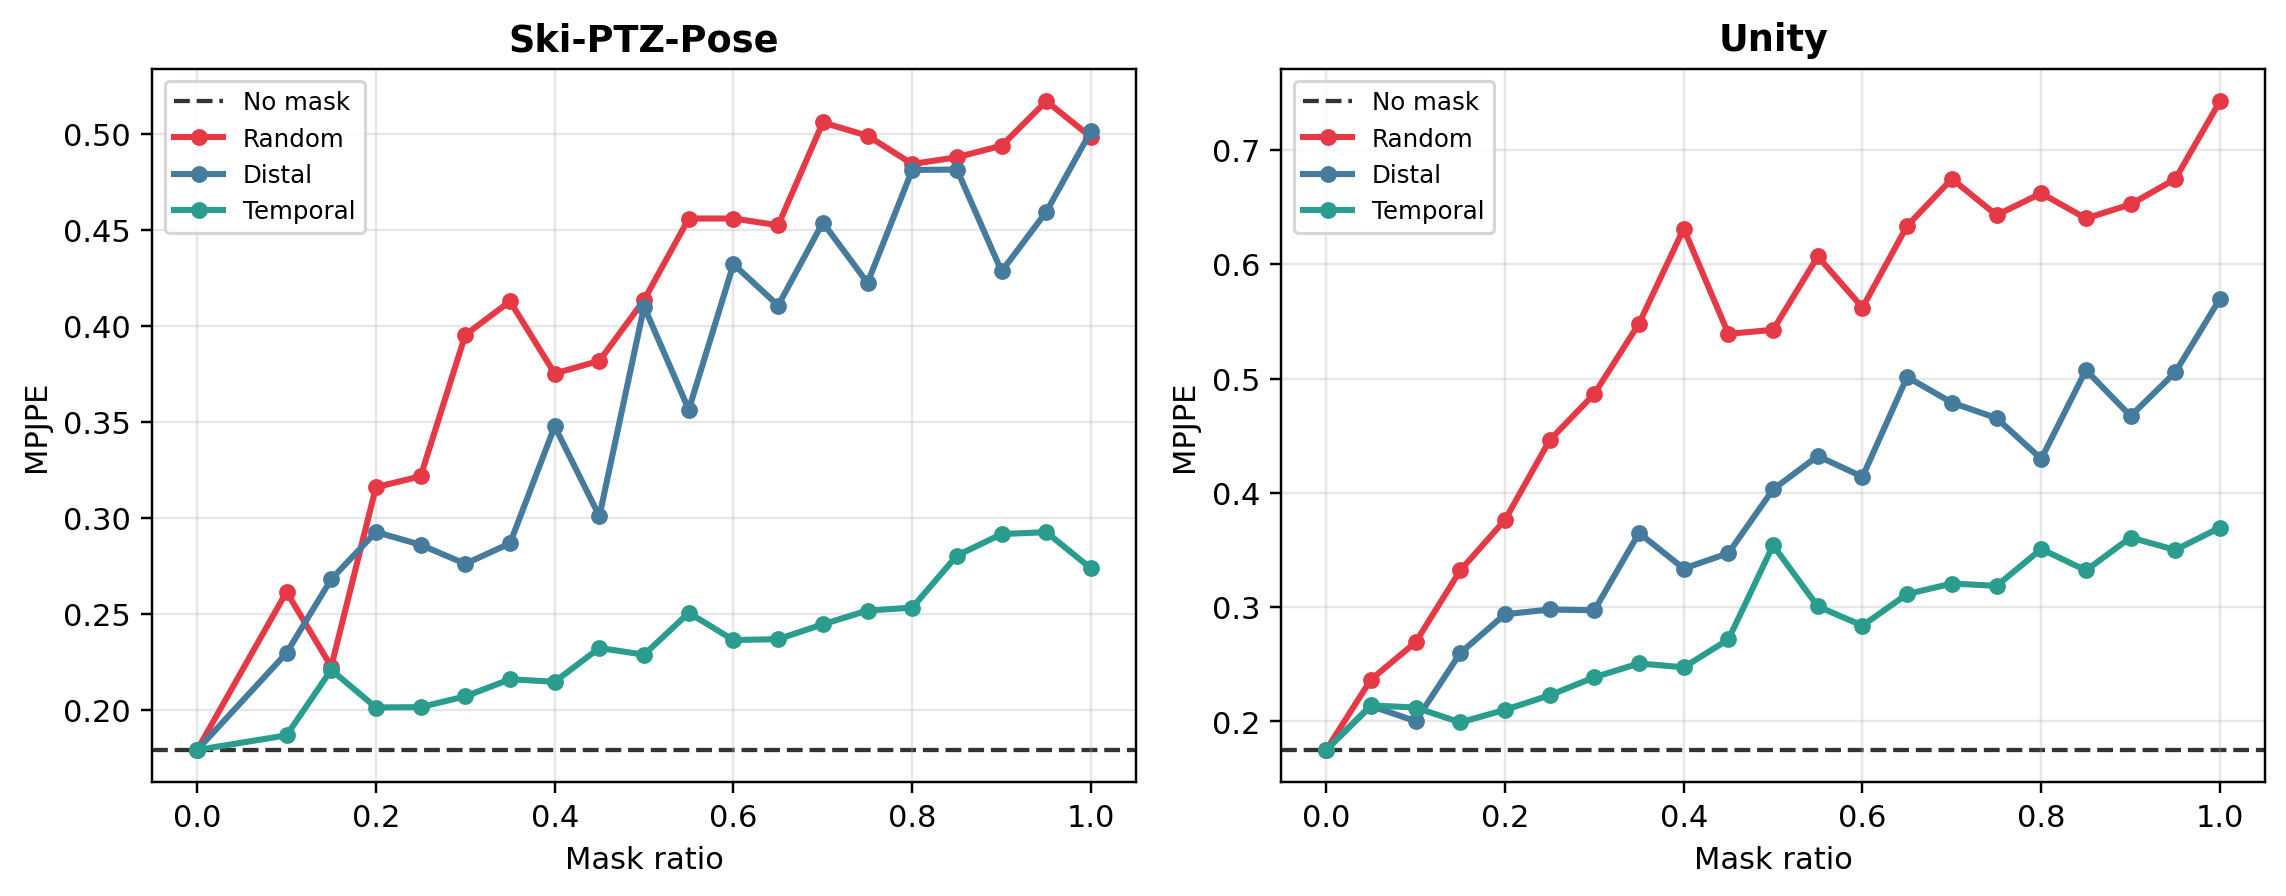
\includegraphics[width=0.98\textwidth]{figure/experiment2/masking_both_view_trends.png}
\caption{Both-view masking robustness on Ski-PTZ-Pose and Unity. Curves show MPJPE as the masking ratio increases when both pose streams are corrupted under random joint-frame, distal-joint, and temporal masking.}
\Description{Two line charts show MPJPE versus masking ratio for random, distal-joint, and temporal masking on Ski-PTZ-Pose and Unity in the both-view corruption setting.}
\label{fig:masking_robustness}
\end{figure*}

\subsection{Feature Ablation}

Table~\ref{tab:feature_ablation_combined} confirms that aligned opposite-view pose is the most important feature: removing it increases MPJPE from \(0.2711\) to \(0.5145\) on Unity and from \(0.1794\) to \(0.2110\) on Ski-PTZ-Pose. Residual, velocity, and rotation cues provide smaller but complementary gains, showing that cross-view alignment supplies the core evidence while motion and geometric disagreement cues refine joint-level reliability.

The ablation results also clarify the roles of the auxiliary cues. Removing the residual feature has a limited effect on Unity but a larger effect on Ski-PTZ-Pose, suggesting that residual disagreement is more useful when real videos contain stronger view-dependent estimation errors. Velocity and rotation cues produce smaller changes in MPJPE, but they help encode whether a disagreement is consistent with plausible motion or is likely to be a transient pose error. These results support the design choice of combining pose-level alignment with lightweight motion-aware features rather than relying on a single global fusion rule.

\begin{table*}[!t]
\centering
\caption{Feature ablation on Unity and Ski-PTZ-Pose. Lower MPJPE is better.}
\label{tab:feature_ablation_combined}
\footnotesize
\setlength{\tabcolsep}{3.5pt}
\renewcommand{\arraystretch}{1.03}
\begin{tabular}{lccccc|cc}
\hline
Variant
& Own
& Aligned
& Residual
& Velocity
& Rot. cue
& Unity MPJPE \(\downarrow\)
& Ski-PTZ MPJPE \(\downarrow\) \\
\hline
Full model
& \checkmark & \checkmark & \checkmark & \checkmark & \checkmark
& \textbf{0.2711} & \textbf{0.1794} \\

w/o aligned pose
& \checkmark & -- & \checkmark & \checkmark & \checkmark
& 0.5145 & 0.2110 \\

w/o residual
& \checkmark & \checkmark & -- & \checkmark & \checkmark
& 0.2728 & 0.1898 \\

w/o velocity
& \checkmark & \checkmark & \checkmark & -- & \checkmark
& 0.2726 & 0.1804 \\

w/o rotation cue
& \checkmark & \checkmark & \checkmark & \checkmark & --
& 0.2853 & 0.1825 \\

w/o residual + rotation cue
& \checkmark & \checkmark & -- & \checkmark & --
& 0.2877 & 0.1943 \\
\hline
Canonical average
& \checkmark & -- & -- & -- & --
& 0.3705 & 0.3487 \\
\hline
\end{tabular}
\end{table*}

\subsection{Real-World Qualitative Evaluation}

\begin{figure*}[!t]
\centering
\begin{minipage}{0.49\textwidth}
\centering
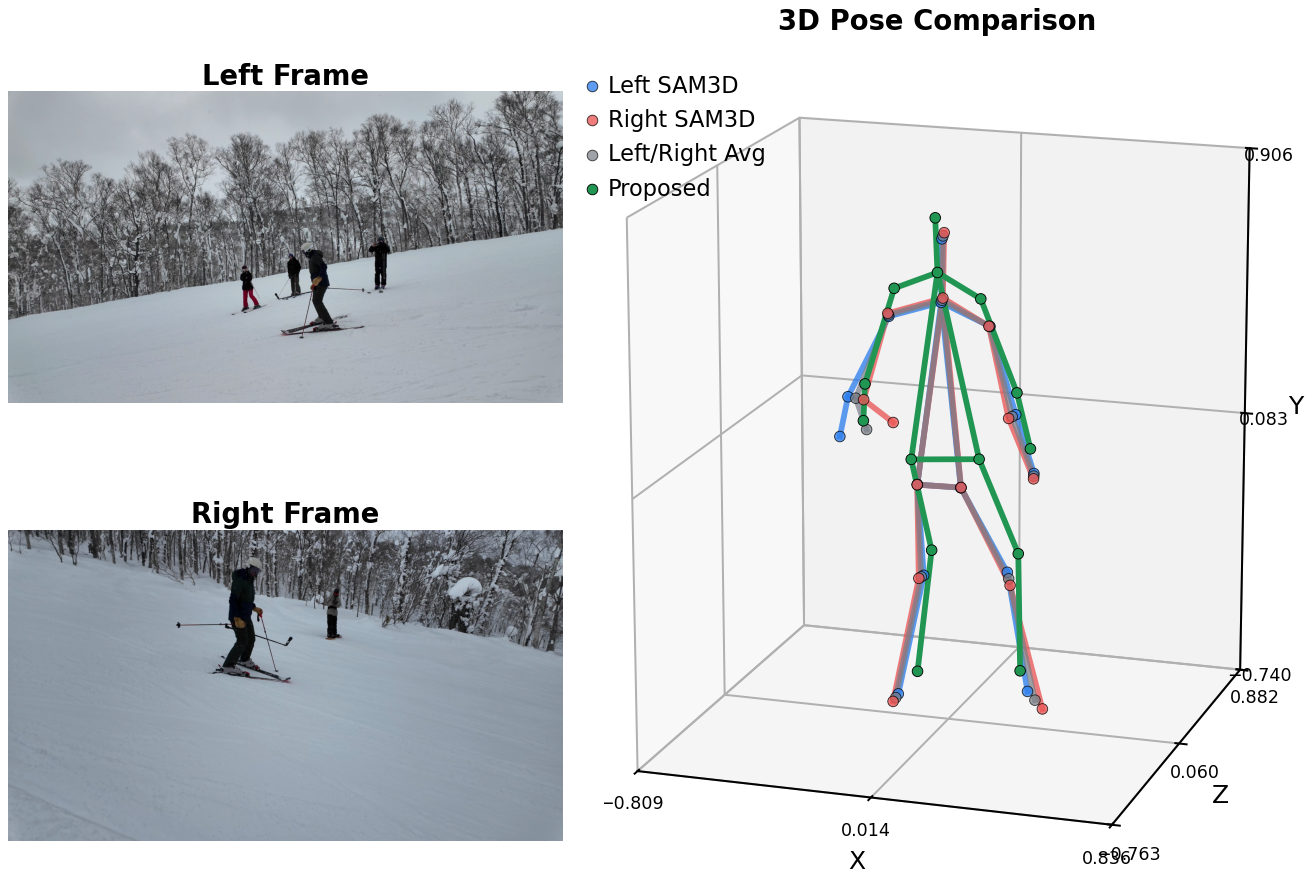
\includegraphics[width=\linewidth]{figure/experiment3/pro_1_frame0000_real_compare.png}
\vspace{-1mm}
\centerline{(a) Outdoor skiing example}
\end{minipage}
\hfill
\begin{minipage}{0.49\textwidth}
\centering
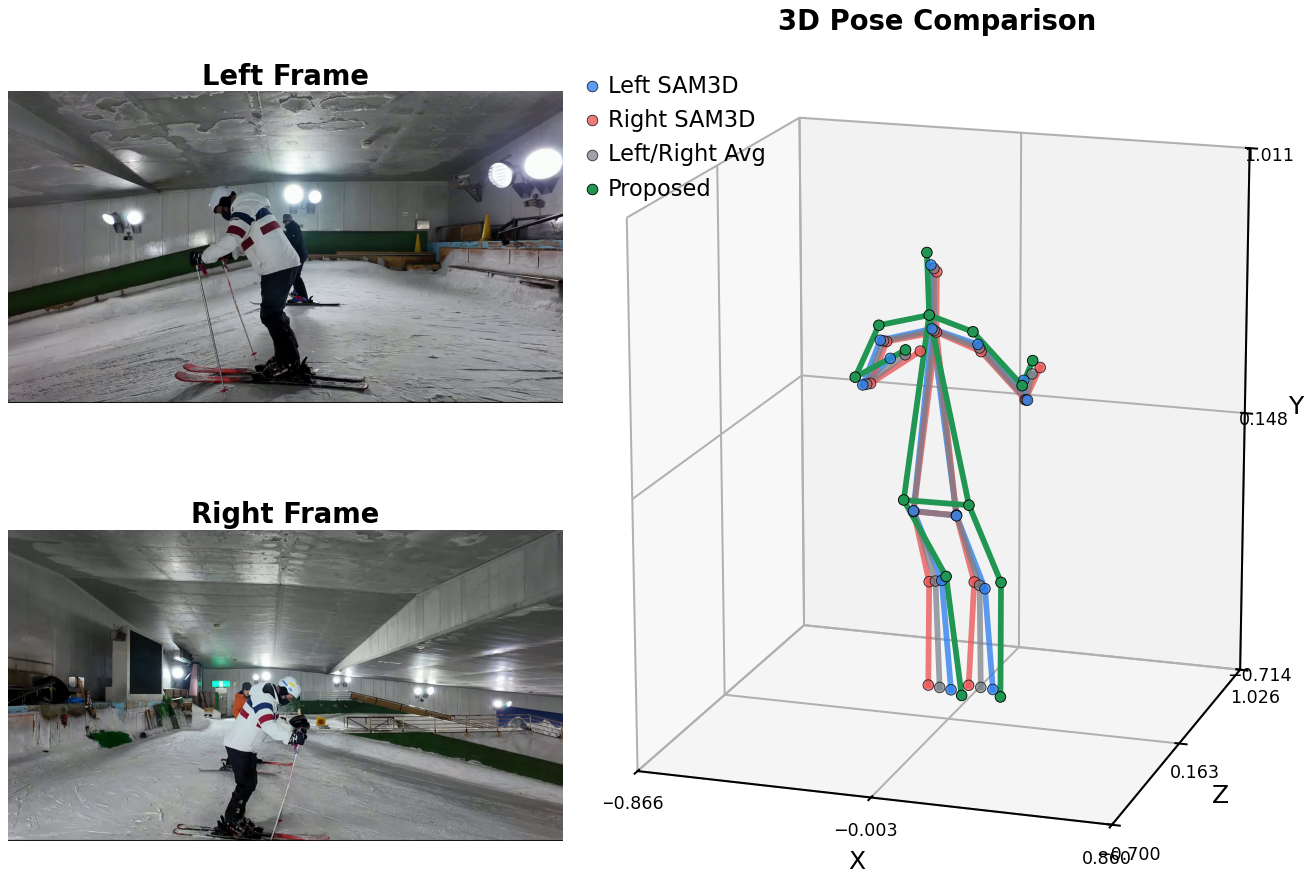
\includegraphics[width=\linewidth]{figure/experiment3/run_3_frame0000_real_compare.png}
\vspace{-1mm}
\centerline{(b) Indoor skiing example}
\end{minipage}
\caption{Qualitative comparison on real skiing videos. Blue/red are single-view predictions, gray is direct average, and green is the proposed refinement.}
\Description{Two qualitative examples compare left-view and right-view pose predictions, direct average fusion, and the proposed refined pose for outdoor and indoor skiing videos.}
\label{fig:real_world_comparison}
\end{figure*}

Figure~\ref{fig:real_world_comparison} illustrates deployment on real skiing videos, where left- and right-view poses are estimated independently and no camera calibration is used during inference. The proposed result remains more coherent than either single-view prediction or direct averaging, especially when the two views disagree around arms, knees, and feet. The examples also show the main limitation: if both upstream predictions contain similar errors, the refinement can still inherit part of that error.

Qualitatively, the refined skeleton tends to preserve the more stable limb configuration while avoiding abrupt compromises caused by direct averaging. This is particularly visible in poses with strong torso rotation, occluded lower limbs, or large differences between left- and right-view predictions. For sports analysis, such behavior is useful because downstream measures such as joint-angle trajectories, limb extension timing, and motion smoothness are sensitive to frame-level outliers. At the same time, the examples should be read as a post-estimation refinement result rather than as full 3D reconstruction from images; the method improves the consistency of available pose streams but does not recover information that is absent from both inputs.

\paragraph{Experimental limitations.}
The experiments have three main limitations. First, Unity uses a recorded avatar skeleton, while Ski-PTZ-Pose uses a fused canonical reference; its numbers therefore measure canonical-reference agreement rather than independent physical 3D accuracy. Second, because the method refines upstream pose streams, it may inherit errors when both monocular estimates fail similarly. Third, all experiments assume synchronized dual-view streams, and temporal camera offsets remain unevaluated.

\section{Conclusion}
\label{sec:conclusion}

This paper presented a calibration-free dual-view 3D pose refinement framework for sports motion analysis. Instead of estimating 3D pose directly from images or relying on full multi-view camera calibration, the proposed method operates on two independently estimated 3D pose streams. By combining body-centric canonicalization, pose-level cross-view alignment, bidirectional cross-view attention, temporal refinement, reliability-gated fusion, and residual correction, the framework refines noisy dual-view pose sequences into more accurate and temporally stable 3D motion trajectories.

Experiments on the Unity synthetic dataset and Ski-PTZ-Pose show that the proposed method improves over single-view inputs and simple fusion baselines in canonical pose space. Unity is evaluated against the recorded avatar skeleton, whereas Ski-PTZ-Pose is evaluated against the fused canonical reference pose and should be interpreted as reference agreement rather than independent motion-capture accuracy. The robustness analysis further demonstrates that the model degrades more gracefully under masked 3D pose inputs, and the acceleration-error results indicate improved temporal consistency in the evaluated canonical space.

Future work will extend the framework to more sports categories, more camera views, stronger long-range temporal modeling, temporal-offset robustness, and uncertainty calibration for more interpretable reliability estimation.

\begin{acks}

We thank the dataset providers and the open-source research community for making this work possible.
This research, in part, used computational resources of Pegasus provided by the Multidisciplinary Cooperative Research Program in the Center for Computational Sciences, University of Tsukuba.
This work used computational resources of Pegasus provided by University of Tsukuba through the HPCI System Research Project (Project ID: hp260146).
\end{acks}


% \clearpage
%%
%% The next two lines define the bibliography style to be used, and
%% the bibliography file.
\bibliographystyle{ACM-Reference-Format}
\bibliography{sample-base}


%%
%% If your work has an appendix, this is the place to put it.
\appendix

% \section{Research Methods}

% \subsection{Part One}

% Lorem ipsum dolor sit amet, consectetur adipiscing elit. Morbi
% malesuada, quam in pulvinar varius, metus nunc fermentum urna, id
% sollicitudin purus odio sit amet enim. Aliquam ullamcorper eu ipsum
% vel mollis. Curabitur quis dictum nisl. Phasellus vel semper risus, et
% lacinia dolor. Integer ultricies commodo sem nec semper.

% \subsection{Part Two}

% Etiam commodo feugiat nisl pulvinar pellentesque. Etiam auctor sodales
% ligula, non varius nibh pulvinar semper. Suspendisse nec lectus non
% ipsum convallis congue hendrerit vitae sapien. Donec at laoreet
% eros. Vivamus non purus placerat, scelerisque diam eu, cursus
% ante. Etiam aliquam tortor auctor efficitur mattis.

% \section{Online Resources}

% Nam id fermentum dui. Suspendisse sagittis tortor a nulla mollis, in
% pulvinar ex pretium. Sed interdum orci quis metus euismod, et sagittis
% enim maximus. Vestibulum gravida massa ut felis suscipit
% congue. Quisque mattis elit a risus ultrices commodo venenatis eget
% dui. Etiam sagittis eleifend elementum.

% Nam interdum magna at lectus dignissim, ac dignissim lorem
% rhoncus. Maecenas eu arcu ac neque placerat aliquam. Nunc pulvinar
% massa et mattis lacinia.

\end{document}
\endinput
%%
%% End of file `sample-sigplan.tex'.
